\documentclass[]{article}
\usepackage{lmodern}
\usepackage{amssymb,amsmath}
\usepackage{ifxetex,ifluatex}
\usepackage{fixltx2e} % provides \textsubscript
\ifnum 0\ifxetex 1\fi\ifluatex 1\fi=0 % if pdftex
  \usepackage[T1]{fontenc}
  \usepackage[utf8]{inputenc}
\else % if luatex or xelatex
  \ifxetex
    \usepackage{mathspec}
  \else
    \usepackage{fontspec}
  \fi
  \defaultfontfeatures{Ligatures=TeX,Scale=MatchLowercase}
\fi
% use upquote if available, for straight quotes in verbatim environments
\IfFileExists{upquote.sty}{\usepackage{upquote}}{}
% use microtype if available
\IfFileExists{microtype.sty}{%
\usepackage{microtype}
\UseMicrotypeSet[protrusion]{basicmath} % disable protrusion for tt fonts
}{}
\usepackage[margin=1in]{geometry}
\usepackage{hyperref}
\hypersetup{unicode=true,
            pdftitle={Testing eyewitness data against the Block-Marschak inequalities},
            pdfauthor={Kym McCormick},
            pdfborder={0 0 0},
            breaklinks=true}
\urlstyle{same}  % don't use monospace font for urls
\usepackage{graphicx,grffile}
\makeatletter
\def\maxwidth{\ifdim\Gin@nat@width>\linewidth\linewidth\else\Gin@nat@width\fi}
\def\maxheight{\ifdim\Gin@nat@height>\textheight\textheight\else\Gin@nat@height\fi}
\makeatother
% Scale images if necessary, so that they will not overflow the page
% margins by default, and it is still possible to overwrite the defaults
% using explicit options in \includegraphics[width, height, ...]{}
\setkeys{Gin}{width=\maxwidth,height=\maxheight,keepaspectratio}
\IfFileExists{parskip.sty}{%
\usepackage{parskip}
}{% else
\setlength{\parindent}{0pt}
\setlength{\parskip}{6pt plus 2pt minus 1pt}
}
\setlength{\emergencystretch}{3em}  % prevent overfull lines
\providecommand{\tightlist}{%
  \setlength{\itemsep}{0pt}\setlength{\parskip}{0pt}}
\setcounter{secnumdepth}{0}
% Redefines (sub)paragraphs to behave more like sections
\ifx\paragraph\undefined\else
\let\oldparagraph\paragraph
\renewcommand{\paragraph}[1]{\oldparagraph{#1}\mbox{}}
\fi
\ifx\subparagraph\undefined\else
\let\oldsubparagraph\subparagraph
\renewcommand{\subparagraph}[1]{\oldsubparagraph{#1}\mbox{}}
\fi

%%% Use protect on footnotes to avoid problems with footnotes in titles
\let\rmarkdownfootnote\footnote%
\def\footnote{\protect\rmarkdownfootnote}

%%% Change title format to be more compact
\usepackage{titling}

% Create subtitle command for use in maketitle
\providecommand{\subtitle}[1]{
  \posttitle{
    \begin{center}\large#1\end{center}
    }
}

\setlength{\droptitle}{-2em}

  \title{Testing eyewitness data against the Block-Marschak inequalities}
    \pretitle{\vspace{\droptitle}\centering\huge}
  \posttitle{\par}
    \author{Kym McCormick}
    \preauthor{\centering\large\emph}
  \postauthor{\par}
      \predate{\centering\large\emph}
  \postdate{\par}
    \date{3 May 2019}


\begin{document}
\maketitle

\subsection{Demographics}\label{demographics}

\begin{verbatim}
##    vars    n  mean    sd median trimmed   mad min max range skew kurtosis
## X1    1 2718 38.37 11.65     35   37.18 10.38  18  81    63 0.87     0.14
##      se
## X1 0.22
\end{verbatim}

\begin{verbatim}
## $demographics_gender
## .
##                  female        male       other 
## 0.000000000 0.494849154 0.502943341 0.002207506 
## 
## $demographics_country
## .
##                American Samoa      Australia         Brazil         Canada 
##              0              0              0              0              0 
##          China       Colombia          India      Indonesia          Nepal 
##              0              0              0              0              0 
##       Pakistan    Philippines    Puerto Rico        Uruguay            USA 
##              0              0              0              0              1 
##     Uzbekistan     Bangladesh        Germany          Italy        Jamaica 
##              0              0              0              0              0 
##    Netherlands        Romania      Venezuela 
##              0              0              0
\end{verbatim}

\subsection{m-AFC Data}\label{m-afc-data}

NB that each lineup size (m = 2:8) has a different number of
observations.

Vector of correct and incorrect response counts for each lineup size.

\begin{verbatim}
##  [1] 296  38 262  82 223 108 209 113 185 145 182 149 365 361
\end{verbatim}

Vector of CIDs for each lineup size

\begin{verbatim}
## [1] 0.8862275 0.7616279 0.6737160 0.6490683 0.5606061 0.5498489 0.5027548
\end{verbatim}

\subsection{Fit Block-Marschak}\label{fit-block-marschak}

\subsubsection{inequality matrix}\label{inequality-matrix}

\begin{verbatim}
##       max 2AFC 3AFC 4AFC 5AFC 6AFC 7AFC 8AFC        RHS
##  [1,]   2    1    0    0    0    0    0    0  0.5000000
##  [2,]   3    0    1    0    0    0    0    0  0.3333333
##  [3,]   4    0    0    1    0    0    0    0  0.2500000
##  [4,]   5    0    0    0    1    0    0    0  0.2000000
##  [5,]   6    0    0    0    0    1    0    0  0.1666667
##  [6,]   7    0    0    0    0    0    1    0  0.1428571
##  [7,]   8    0    0    0    0    0    0    1  0.1250000
##  [8,]   2   -1    0    0    0    0    0    0 -1.0000000
##  [9,]   3    0   -1    0    0    0    0    0 -1.0000000
## [10,]   4    0    0   -1    0    0    0    0 -1.0000000
## [11,]   5    0    0    0   -1    0    0    0 -1.0000000
## [12,]   6    0    0    0    0   -1    0    0 -1.0000000
## [13,]   7    0    0    0    0    0   -1    0 -1.0000000
## [14,]   8    0    0    0    0    0    0   -1 -1.0000000
## [15,]   3    1   -1    0    0    0    0    0  0.0000000
## [16,]   4    0    1   -1    0    0    0    0  0.0000000
## [17,]   5    0    0    1   -1    0    0    0  0.0000000
## [18,]   6    0    0    0    1   -1    0    0  0.0000000
## [19,]   7    0    0    0    0    1   -1    0  0.0000000
## [20,]   8    0    0    0    0    0    1   -1  0.0000000
## [21,]   4    1   -2    1    0    0    0    0  0.0000000
## [22,]   5    0    1   -2    1    0    0    0  0.0000000
## [23,]   6    0    0    1   -2    1    0    0  0.0000000
## [24,]   7    0    0    0    1   -2    1    0  0.0000000
## [25,]   8    0    0    0    0    1   -2    1  0.0000000
## [26,]   5    1   -3    3   -1    0    0    0  0.0000000
## [27,]   6    0    1   -3    3   -1    0    0  0.0000000
## [28,]   7    0    0    1   -3    3   -1    0  0.0000000
## [29,]   8    0    0    0    1   -3    3   -1  0.0000000
## [30,]   6    1   -4    6   -4    1    0    0  0.0000000
## [31,]   7    0    1   -4    6   -4    1    0  0.0000000
## [32,]   8    0    0    1   -4    6   -4    1  0.0000000
## [33,]   7    1   -5   10  -10    5   -1    0  0.0000000
## [34,]   8    0    1   -5   10  -10    5   -1  0.0000000
## [35,]   8    1   -6   15  -20   15   -6    1  0.0000000
## [36,]   3   -2    1    0    0    0    0    0 -1.0000000
## [37,]   4   -3    3   -1    0    0    0    0 -1.0000000
## [38,]   5   -4    6   -4    1    0    0    0 -1.0000000
## [39,]   6   -5   10  -10    5   -1    0    0 -1.0000000
## [40,]   7   -6   15  -20   15   -6    1    0 -1.0000000
## [41,]   8   -7   21  -35   35  -21    7   -1 -1.0000000
## [42,]  -1    0    0    0    0    0   -7    8  0.0000000
## [43,]  -1    0    0    0    0  -21   49  -28  0.0000000
## [44,]  -1    0    0    0  -35  126 -147   56  0.0000000
## [45,]  -1    0    0  -35  175 -315  245  -70  0.0000000
## [46,]  -1    0  -21  140 -350  420 -245   56  0.0000000
## [47,]  -1   -7   63 -210  350 -315  147  -28  0.0000000
## [48,]  -1   14  -63  140 -175  126  -49    8  1.0000000
\end{verbatim}

\subsubsection{Fitting to the Block Marschak
inequalities}\label{fitting-to-the-block-marschak-inequalities}

Closest fitting expected data that respect the Block-Marschak
inequalities:

\begin{verbatim}
## [1] 0.8711353 0.7687420 0.6885933 0.6264624 0.5781227 0.5393473 0.5059095
\end{verbatim}

\subsubsection{Fitting to the Block-Marschak inequalities (with
monotonic likelihood constraint
applied)}\label{fitting-to-the-block-marschak-inequalities-with-monotonic-likelihood-constraint-applied}

Closest fitting expected data that respect the Block-Marschak
inequalities and the monotonic likelihood constraint:

\begin{verbatim}
## [1] 0.8719132 0.7694413 0.6887421 0.6259732 0.5772925 0.5388578 0.5068268
\end{verbatim}

\subsubsection{Yields rankings}\label{yields-rankings}

reconstructing the CID and FID (respectively) from the m-AFC data:

\begin{verbatim}
## [1] 0.5068268 0.7310438 0.8655219 1.0000000 1.0000000 1.0000000 1.0000000
## [8] 1.0000000
\end{verbatim}

\begin{verbatim}
## [1] 0.07045331 0.18127946 0.30492544 0.42857143 0.57142857 0.71428571
## [7] 0.85714286 1.00000000
\end{verbatim}

\subsubsection{G-square:}\label{g-square}

\paragraph{Block- Marschak}\label{block--marschak}

\begin{verbatim}
## [1] 2.43665
\end{verbatim}

\paragraph{Block-Marschak with monotonic
likelihood}\label{block-marschak-with-monotonic-likelihood}

\begin{verbatim}
## [1] 2.421121
\end{verbatim}

\subsubsection{Multiplicative
inequalities}\label{multiplicative-inequalities}

\begin{verbatim}
## [1] TRUE
\end{verbatim}

Therefore, G-Square equal to 0, p-value equal to 1.

\subsubsection{Bootstrap p-value}\label{bootstrap-p-value}

Block-Marschak inequalities:

\begin{verbatim}
## [1] 0.65927
\end{verbatim}

Block-Marschak inequalities with monotonic likelihood constraint:

\begin{verbatim}
## [1] 0.70868
\end{verbatim}

\subsection{Figure}\label{figure}

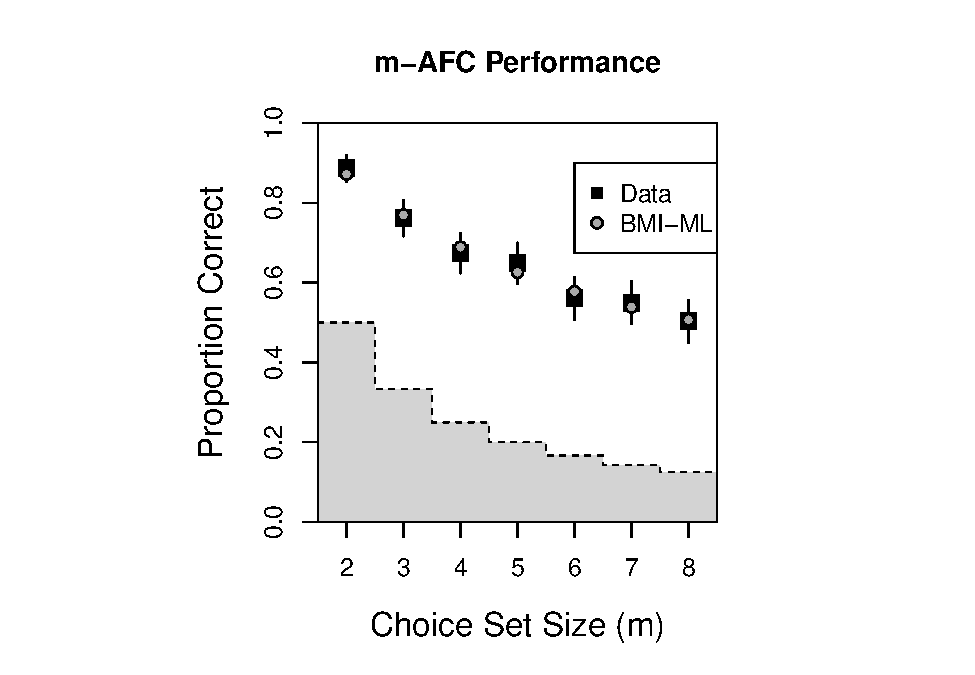
\includegraphics{b_m_output_files/figure-latex/unnamed-chunk-13-1.pdf}

\subsection{Reconstructed eyewitness identification
ROC}\label{reconstructed-eyewitness-identification-roc}

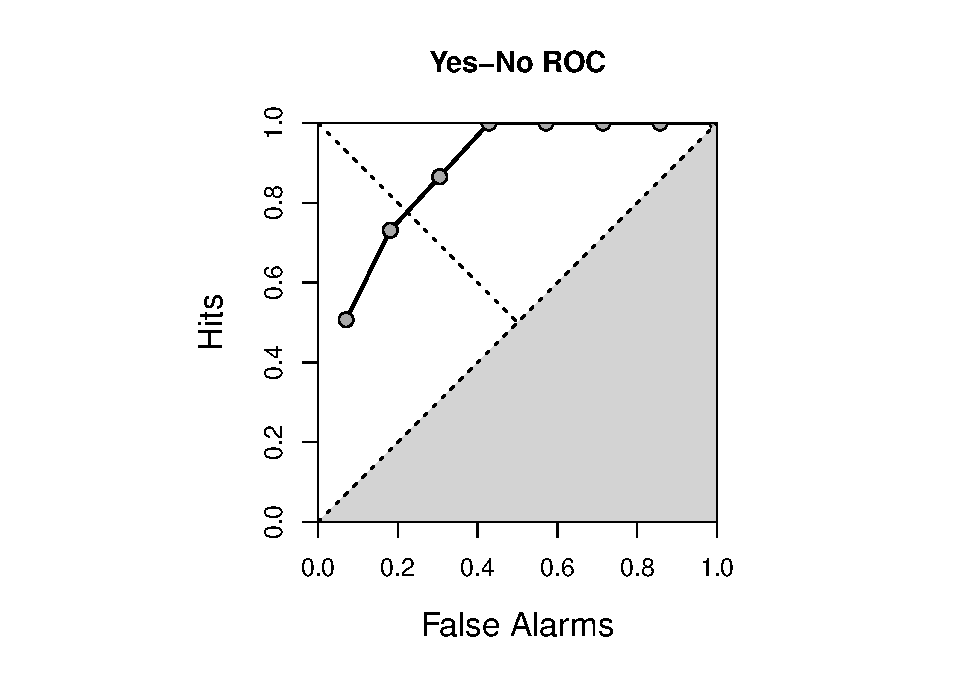
\includegraphics{b_m_output_files/figure-latex/unnamed-chunk-14-1.pdf}


\end{document}
